\section{Open-loop planning via H-steps ahead predictions}
\label{sec:open_loop_planning}
In this section, we address the problem of planning under uncertainty for a stochastic system.
At each grid point $k$ of the discretized trajectory the covariance matrix is propagated in a feed-forward fashion for a fixed prediction horizon of $H$ steps.
In the planning problem, we conservatively evaluate the maximum propagation of the covariance, that is, the matrix evolved over $H$ steps, to ensure the tightest possible enforcement of constraints. This maximizes the robustness of the resulting solution, as the constraint back-off is evaluated in the worst-case scenario within the prediction horizon.

To enable this, we associate multiple versions of the covariance matrix with each grid point. Specifically, $H+1$ instances of the matrix $\bP$ are maintained at each step. To this sake we introduce the notation $\bP_k^j$, where $j = 0, \ldots, H$, and $\bP_k^j$ represents the version of the covariance matrix at step $k$ that was initialized $j$ steps earlier. Hence, $\bP_k^0$ originates at node $k$ itself and will be propagated forward and employed in subsequent steps (exactly when evolved as $\bP_{k+H}^H$ ), while $\bP_k^H$ is the instance that originated $H$ steps earlier and is the most propagated one at step $k$.

The repeated initialization of the covariance matrix at each step is necessary to prevent its unbounded growth, as we assume that the system evolves without feedback control.
In the absence of feedback, the uncertainty on the position and orientation of the body frame accumulates along the track, leading to a severe and unrealistic degradation of the covariance matrix conditioning.
For this reason, the propagation horizon in this open-loop setting is a critical design parameter.
We bound the number of steps $H$ to realistically capture the evolution of disturbances occurring prior to any corrective driver response.

This approach requires modifications to the formulation~\eqref{eq:DOCP} introduced in Section~\ref{sec:discretization}. In particular, Eqs.~\eqref{eq:DOCPdP}, \eqref{eq:DOCPdPIC}, and \eqref{eq:DOCPconstraints} are replaced by Eqs.~\eqref{eq:DOCPdPopenloop}, \eqref{eq:DOCPdPinitopenloop}, and \eqref{eq:DOCPconstraintsopenloop}. Equation~\eqref{eq:DOCPdPopenloop} collects the continuity and collocation equations for all versions of the covariance matrix propagated from previous steps. To support the evolution of $H$ versions, we introduce $H \times d$ matrices $\bSi_k^j = (\bSi_{k,1}^j, \ldots, \bSi_{k,d}^j)$, representing the collocation values of each version $j$ of the covariance matrix within interval $k$.


%The proposed approach requires the presence of $H+1$ versions of the matrix $\bP$ at each grid point of the discretized problem. One of these versions is initialized with $\bar{\bP}_0$, while the others represent the evolution of matrices that were initialized at previous grid points, from 1 to $H$ steps earlier. This ensures that at each step it is possible to find a covariance matrix evolved for $H$ steps and use it to robustify the constraints. The initialization of the covariance matrix is necessary due to its divergent dynamics. In fact, without a feedback control, the error on the position and orientation of the body reference frame can only increase along the track, compromising the conditioning of the matrix.
%
%Introducing the versioning of the covariance matrix approach requires a modification of the Equations described in Section~\ref{sec:discretization}. In particular Eqs.~\eqref{eq:DOCPdP}, \eqref{eq:DOCPdPIC}, and \eqref{eq:DOCPconstraints} are replaced by Eqs.~\eqref{eq:DOCPdPopenloop}, \eqref{eq:DOCPdPinitopenloop}, and \eqref{eq:DOCPconstraintsopenloop}. Eq.~\eqref{eq:DOCPdPopenloop} collects the continuity and collocation Equations for all the versions of the covariance matrix that have propagated from the previous step. To account for the evolution of $H$ matrices, it is necessary to introduce $H\times d$ matrices $\bSi_k^j=(\bSi_{k,1}^j, \ldots, \bSi_{k,d}^j)$, which represent the values of each matrix version at the collocation points.

The specific formulation is expressed as follows:
\begin{subequations}\label{eq:DOCPopenloop}
\begin{alignat}{3}
	\underset{\bmu_k,\bxi_k, \bu_k, \bP_k,\bz_k}{\text{minimize}} \,
	& & & J_k(\bmu_k,\bxi_k, \bu_k) & & \label{eq:DOCPcostopenloop} \\
	\hspace*{-2.0 cm}\text{s.t.} \quad
	& \bzero      & = & \; \bPsimu_k(\bmu_{k-1},\bmu_k,\bxi_k, \bu_k,\bz_k),
	& \quad & k = 1,\ldots, N \label{eq:DOCPdynopenloop} \\
	& \bmu_0      & = & \; \bar{\bmu}_0
	& & \label{eq:DOCPdynICopenloop} \\
	& \bzero      & = & \; \bPsiP_k(\bmu_k,\bxi_k, \bu_k, \bP_{k-1}^{j-1},\bP_k^j,\bSi_k^j,\bz_k),
	& \quad & \substack{k = 1,\ldots, N; \; \\ j=1,\ldots,H;\;} \label{eq:DOCPdPopenloop} \\
	& \bP_k^0       & = & \; \bar{\bP}_0 \succeq 0
	& \quad & k = 1,\ldots, N; \; \label{eq:DOCPdPinitopenloop} \\
	& \bzero      & = & \; \bOm_k(\bmu_k,\bxi_k, \bu_k,\bz_k),
	& \quad & k = 0,\ldots, N \label{eq:DOCPpathopenloop} \\
	& 0           & \geq & \; h_i(\bmu_k, \bu_k, \bz_k) + \be_i(\bmu_k, \bu_k, \bP_k^H, \bz_k),
	& \quad & k = 1,\ldots, N;\; i \in \calI \label{eq:DOCPconstraintsopenloop}
\end{alignat}
\end{subequations}
Equation~\eqref{eq:DOCPdPinitopenloop} defines the initialization of the appropriate covariance matrix version at step $k$, while Eq.~\eqref{eq:DOCPconstraintsopenloop} specifies that the back-off term in the constraints is computed using the most propagated version, $\bP^H_k$. A schematic illustration of the management of the $H+1$ covariance matrix instances is provided in Fig.~\ref{fig:DOCPgrid}. The dashed rectangle highlights the $k$-th discretization step, where the constraints are evaluated. At each grid point, two particular versions of the covariance matrix are emphasized: $\bP^0_k$ (red node), representing the instance to be initialized at that step, and $\bP^H_k$ (green node), corresponding to the version that has been propagated over the full horizon of $H$ steps and is used to robustify the constraints in Eq.~\eqref{eq:DOCPconstraintsopenloop}.



%Eq.~\eqref{eq:DOCPdPinitopenloop} is used to initialize the correct version at the $k$-th step while Eq.~\eqref{eq:DOCPconstraintsopenloop} specify that the back-off term of the constraints is evaluated with the most propagated covariance matrix version, $\bP^H_k$.
%A schematic representation of the approach used to manage the $H+1$ versions of the covariance matrix is shown in Figure \ref{fig:DOCPgrid}, where the dashed rectangle represent the $k$-th step at which the constraints are being formulated. At each grid point, two versions of the covariance matrix are highlighted: $\bP^0_k$ (red node), which is the version to be initialized, and $\bP^H_k$ (green node), which is the most propagated version used to formulate the robust constraints in Eq.~\eqref{eq:DOCPconstraintsopenloop}.
\def\version{marco}
\ifdefstring{\version}{matteo}{
\begin{figure}
	\centering
	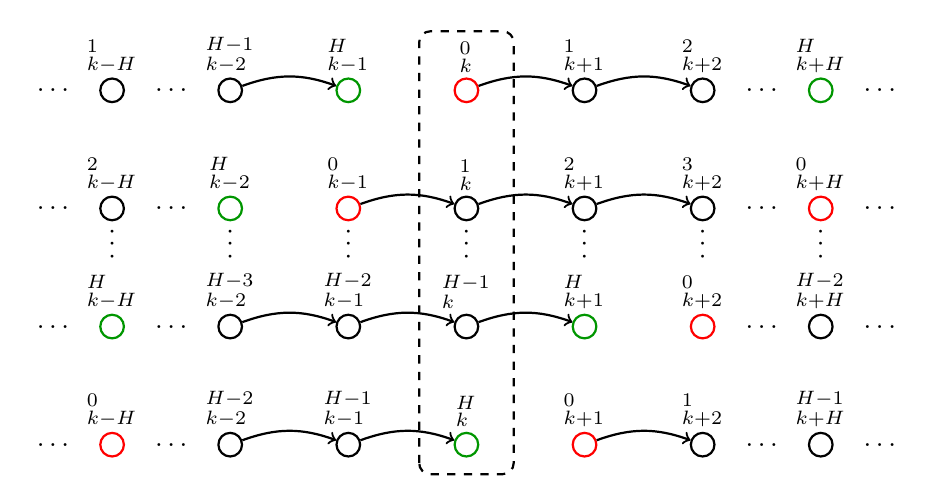
\begin{tikzpicture}[%
	smallnode/.style={%
		circle, draw, minimum size=3mm, inner sep=0pt
	},
	r_smallnode/.style={%
		circle, draw, minimum size=3mm, inner sep=0pt, red
	},
	g_smallnode/.style={%
		circle, draw, minimum size=3mm, inner sep=0pt, mygreen
	},
	every path/.style={->, thick},
	x=1.5cm, y=1.5cm
	]
	
	\newcommand{\Plab}[2]{\bP^{#2}_{#1}}
	\definecolor{mygreen}{RGB}{0 150 0}
	
	% Nodes
	% First row
	\node[smallnode, label={[label distance=-2pt]above:\(\Plab{k-2}{H-2}\)}] (Pk-2H-2) at (1,0) {};
	\node[smallnode, label={[label distance=-2pt]above:\(\Plab{k-1}{H-1}\)}] (Pk-1H-1) at (2,0) {};
	\node[g_smallnode, label={[label distance=-2pt]above:\(\Plab{k}{H}\)}] (PkH) at (3,0) {};
	\node[r_smallnode, label={[label distance=-2pt]above:\(\Plab{k+1}{0}\)}] (Pk+10) at (4,0) {};
	\node[smallnode, label={[label distance=-2pt]above:\(\Plab{k+2}{1}\)}] (Pk+21) at (5,0) {};
	
	\draw[bend left=20] (Pk-2H-2) to (Pk-1H-1);
	\draw[bend left=20] (Pk-1H-1) to (PkH);
	\draw[bend left=20] (Pk+10) to (Pk+21);
	
	\node[r_smallnode, label={[label distance=-2pt]above:\(\Plab{k-H}{0}\)}] (Pk-H0) at (0,0) {};
	\node[label={center:\(\dots\)}] (dots10) at (-.5, 0) {};
	\node[label={center:\(\dots\)}] (dots11) at (.5, 0) {};
	\node[smallnode, label={[label distance=-2pt]above:\(\Plab{k+H}{H-1}\)}] (Pk+HH-1) at (6,0) {};
	\node[label={center:\(\dots\)}] (dots12) at (5.5, 0) {};
	\node[label={center:\(\dots\)}] (dots13) at (6.5, 0) {};
	% Second row
	\node[smallnode, label={[label distance=-2pt]above:\(\Plab{k-2}{H-3}\)}] (Pk-2H-3) at (1,1) {};
	\node[smallnode, label={[label distance=-2pt]above:\(\Plab{k-1}{H-2}\)}] (Pk-1H-2) at (2,1) {};
	\node[smallnode, label={[label distance=-2pt]above:\(\Plab{k}{H-1}\)}] (PkH-1) at (3,1) {};
	\node[g_smallnode, label={[label distance=-2pt]above:\(\Plab{k+1}{H}\)}] (Pk+1H) at (4,1) {};
	\node[r_smallnode, label={[label distance=-2pt]above:\(\Plab{k+2}{0}\)}] (Pk+20) at (5,1) {};
	
	\draw[bend left=20] (Pk-2H-3) to (Pk-1H-2);
	\draw[bend left=20] (Pk-1H-2) to (PkH-1);
	\draw[bend left=20] (PkH-1) to (Pk+1H);
	
	\node[g_smallnode, label={[label distance=-2pt]above:\(\Plab{k-H}{H}\)}] (Pk-HH) at (0,1) {};
	\node[label={center:\(\dots\)}] (dots20) at (-.5, 1) {};
	\node[label={center:\(\dots\)}] (dots21) at (.5, 1) {};
	\node[smallnode, label={[label distance=-2pt]above:\(\Plab{k+H}{H-2}\)}] (Pk+HH-2) at (6,1) {};
	\node[label={center:\(\dots\)}] (dots22) at (5.5, 1) {};
	\node[label={center:\(\dots\)}] (dots23) at (6.5, 1) {};
	
	% dots row
	\node[label={center,rotate=90:\(\dots\)}] (dots1) at (0, 1.7) {};
	\node[label={center,rotate=90:\(\dots\)}] (dots2) at (1, 1.7) {};
	\node[label={center,rotate=90:\(\dots\)}] (dots3) at (2, 1.7) {};
	\node[label={center,rotate=90:\(\dots\)}] (dots4) at (3, 1.7) {};
	\node[label={center,rotate=90:\(\dots\)}] (dots5) at (4, 1.7) {};
	\node[label={center,rotate=90:\(\dots\)}] (dots6) at (5, 1.7) {};
	\node[label={center,rotate=90:\(\dots\)}] (dots7) at (6, 1.7) {};
	
	% Third row
	\node[g_smallnode, label={[label distance=-2pt]above:\(\Plab{k-2}{H}\)}] (Pk-2H) at (1,2) {};
	\node[r_smallnode, label={[label distance=-2pt]above:\(\Plab{k-1}{0}\)}] (Pk-10) at (2,2) {};
	\node[smallnode, label={[label distance=-2pt]above:\(\Plab{k}{1}\)}] (Pk1) at (3,2) {};
	\node[smallnode, label={[label distance=-2pt]above:\(\Plab{k+1}{2}\)}] (Pk+12) at (4,2) {};
	\node[smallnode, label={[label distance=-2pt]above:\(\Plab{k+2}{3}\)}] (Pk+23) at (5,2) {};
	
	\draw[bend left=20] (Pk-10) to (Pk1);
	\draw[bend left=20] (Pk1) to (Pk+12);
	\draw[bend left=20] (Pk+12) to (Pk+23);
	
	\node[smallnode, label={[label distance=-2pt]above:\(\Plab{k-H}{2}\)}] (Pk-H2) at (0,2) {};
	\node[label={center:\(\dots\)}] (dots30) at (-.5, 2) {};
	\node[label={center:\(\dots\)}] (dots31) at (.5, 2) {};
	\node[r_smallnode, label={[label distance=-2pt]above:\(\Plab{k+H}{0}\)}] (Pk+H0) at (6,2) {};
	\node[label={center:\(\dots\)}] (dots32) at (5.5, 2) {};
	\node[label={center:\(\dots\)}] (dots33) at (6.5, 2) {};
	
	% Fourth row
	\node[smallnode, label={[label distance=-2pt]above:\(\Plab{k-2}{H-1}\)}] (Pk-2H-1) at (1,3) {};
	\node[g_smallnode, label={[label distance=-2pt]above:\(\Plab{k-1}{H}\)}] (Pk-1H) at (2,3) {};
	\node[r_smallnode, label={[label distance=-2pt]above:\(\Plab{k}{0}\)}] (Pk0) at (3,3) {};
	\node[smallnode, label={[label distance=-2pt]above:\(\Plab{k+1}{1}\)}] (Pk+11) at (4,3) {};
	\node[smallnode, label={[label distance=-2pt]above:\(\Plab{k+2}{2}\)}] (Pk+22) at (5,3) {};
	
	\draw[bend left=20] (Pk-2H-1) to (Pk-1H);
	\draw[bend left=20] (Pk0) to (Pk+11);
	\draw[bend left=20] (Pk+11) to (Pk+22);
	
	\node[smallnode, label={[label distance=-2pt]above:\(\Plab{k-H}{1}\)}] (Pk-H1) at (0,3) {};
	\node[label={center:\(\dots\)}] (dots40) at (-.5, 3) {};
	\node[label={center:\(\dots\)}] (dots41) at (.5, 3) {};
	\node[g_smallnode, label={[label distance=-2pt]above:\(\Plab{k+H}{H}\)}] (Pk+HH) at (6,3) {};
	\node[label={center:\(\dots\)}] (dots42) at (5.5, 3) {};
	\node[label={center:\(\dots\)}] (dots43) at (6.5, 3) {};
	
	% Dashed rectangle
	\draw[dashed, thick, rounded corners] (2.6,-.25) rectangle (3.4,3.5);
	
\end{tikzpicture}
	\caption{Schematic representation of the continuity and initialization equations associated with the $H+1$ propagated instances of the covariance matrix introduced in problem~\eqref{eq:DOCPopenloop}. The dashed rectangle highlights the $k$-th discretization step, at which the robust constraints are enforced. Each node corresponds to a specific covariance matrix, where the subscript denotes the current grid index and the superscript indicates the number of propagation steps since initialization. At each step, two key instances are emphasized: the matrix to be initialized at that step (red node), and the matrix that has been propagated over $H$ steps (green node), which is used in the evaluation of the constraint backoff.}
	%\caption{Schematic representation of the continuity and initialization Equations for the $H+1$ versions of the covariance matrix introduced in the discretized OCP. The dashed rectangle indicate the $k$-th step, in which the constraints are formulated. Each node represents a covariance matrix, labeled such that the subscript denotes the current grid step, while the superscript indicates the number of propagation steps it has undergone. At each step, two nodes are highlighted: the covariance matrix to be initialized (red node) and the matrix that has been propagated for $H$ steps (green node), which is used to formulate the robust constraints.}
	\label{fig:DOCPgrid}
\end{figure}
}{}

\ifdefstring{\version}{marco}{
\begin{figure}
	\centering
	\definecolor{mygreen}{RGB}{0,150,0}
	\begin{tikzpicture}[
	smallnode/.style={circle, draw, minimum size=3mm, inner sep=0pt},
	r_smallnode/.style={circle, draw=red, minimum size=3mm, inner sep=0pt},
	g_smallnode/.style={circle, draw=mygreen, minimum size=3mm, inner sep=0pt},
	r_hatnode/.style={
		circle, draw=red, pattern=north east lines, pattern color=red,
		minimum size=3mm, inner sep=0pt},
	g_hatnode/.style={
		circle, draw=mygreen, pattern=north east lines, pattern color=mygreen,
		minimum size=3mm, inner sep=0pt},
	every path/.style={->, thick},
	x=1.4cm, y=1.2cm
	]
	
	% ROW j = 0 (y=3)
	\node[r_hatnode, label={[label distance=-2pt]above:\(\bP_{k-3}^0\)}] (P00) at (1,3) {};
	\node[smallnode, label={[label distance=-2pt]above:\(\bP_{k-2}^1\)}] (P11) at (2,3) {};
	\node[smallnode, label={[label distance=-2pt]above:\(\bP_{k-1}^2\)}] (P22) at (3,3) {};
	\node[g_hatnode, label={[label distance=-2pt]above:\(\bP_k^3\)}] (P33) at (4,3) {};
	\node[r_hatnode, label={[label distance=-2pt]above:\(\bP_{k+1}^0\)}] (P44) at (5,3) {};
	\node[smallnode, label={[label distance=-2pt]above:\(\bP_{k+2}^1\)}] (P55) at (6,3) {};
	
	% ROW j = 1 (y=2)
	\node[r_hatnode, label={[label distance=-2pt]above:\(\bP_{k-2}^0\)}] (P10) at (2,2) {};
	\node[smallnode, label={[label distance=-2pt]above:\(\bP_{k-1}^1\)}] (P21) at (3,2) {};
	\node[smallnode, label={[label distance=-2pt]above:\(\bP_k^2\)}] (P32) at (4,2) {};
	\node[g_hatnode, label={[label distance=-2pt]above:\(\bP_{k+1}^3\)}] (P43) at (5,2) {};
	\node[r_hatnode, label={[label distance=-2pt]above:\(\bP_{k+2}^0\)}] (P54) at (6,2) {};
	\node[smallnode, label={[label distance=-2pt]above:\(\bP_{k+3}^1\)}] (P65) at (7,2) {};
	
	
	% ROW j = 2 (y=1)
	\node[r_hatnode, label={[label distance=-2pt]above:\(\bP_{k-1}^0\)}] (P20) at (3,1) {};
	\node[smallnode, label={[label distance=-2pt]above:\(\bP_k^1\)}] (P31) at (4,1) {};
	\node[smallnode, label={[label distance=-2pt]above:\(\bP_{k+1}^2\)}] (P42) at (5,1) {};
	\node[g_hatnode, label={[label distance=-2pt]above:\(\bP_{k+2}^3\)}] (P53) at (6,1) {};
	\node[r_hatnode, label={[label distance=-2pt]above:\(\bP_{k+3}^0\)}] (P64) at (7,1) {};
	\node[smallnode, label={[label distance=-2pt]above:\(\bP_{k+4}^1\)}] (P75) at (8,1) {};
	
	% ROW j = 3 (y=0)
	\node[r_hatnode, label={[label distance=-2pt]above:\(\bP_k^0\)}] (P30) at (4,0) {};
	\node[smallnode, label={[label distance=-2pt]above:\(\bP_{k+1}^1\)}] (P41) at (5,0) {};
	\node[smallnode, label={[label distance=-2pt]above:\(\bP_{k+2}^2\)}] (P52) at (6,0) {};
	\node[g_hatnode, label={[label distance=-2pt]above:\(\bP_{k+3}^3\)}] (P63) at (7,0) {};
	\node[r_hatnode, label={[label distance=-2pt]above:\(\bP_{k+4}^0\)}] (P74) at (8,0) {};
	\node[smallnode, label={[label distance=-2pt]above:\(\bP_{k+5}^1\)}] (P85) at (9,0) {};
	
	
	% ARROWS
	\draw (P00) -- (P11);
	\draw (P11) -- (P22);
	\draw (P22) -- (P33);
	\draw (P22) -- (P33);
	
	\draw (P44) -- (P55);
	\draw[dashed,->] (P55) -- ++(1,0);
	
	\draw (P10) -- (P21);
	\draw (P21) -- (P32);
	\draw (P32) -- (P43);
	\draw (P54) -- (P65);
	\draw[dashed,->] (P65) -- ++(1,0);
	
	
	\draw (P20) -- (P31);
	\draw (P31) -- (P42);
	\draw (P42) -- (P53);
	\draw (P64) -- (P75);
	\draw[dashed,->] (P75) -- ++(1,0);
	
	\draw (P30) -- (P41);
	\draw (P41) -- (P52);
	\draw (P52) -- (P63);
	
	\draw (P74) -- (P85);
	\draw[dashed,->] (P85) -- ++(1,0);
	
	% Dashed box around column k (x=4)
	\draw[dashed, thick, rounded corners] (3.6,-0.5) rectangle (4.4,3.7);
	
	% Top axis labels
	\node at (0, 4.3) {\scriptsize \(\cdots\)};
	\node at (1, 4.3) {\scriptsize \(k-3\)};
	\node at (2, 4.3) {\scriptsize \(k-2\)};
	\node at (3, 4.3) {\scriptsize \(k-1\)};
	\node (knode) at (4, 4.3) {\scriptsize \(k\)};
	\node at (5, 4.3) {\scriptsize \(k+1\)};
	\node at (6, 4.3) {\scriptsize \(k+2\)};
	\node at (7, 4.3) {\scriptsize \(k+3\)};
	\node at (8, 4.3) {\scriptsize \(k+4\)};
	\node at (9, 4.3) {\scriptsize \(\cdots\)};
	
	% Wiggly arrow from label to top edge of dashed box
	\draw[->, thick, decorate, decoration={snake, amplitude=0.25mm, segment length=2.5mm}]
	(knode.south) -- (4, 3.8);
	
	% Legend box (top right)
	%\begin{scope}[shift={(6.5,2.5)}]
	%    \node[r_smallnode] (r) at (0,0) {};
	%    \node[anchor=west] at (0.4,0) {\scriptsize Initialized matrix \(\bP_k^0\)};
	%
	%    \node[g_smallnode] (g) at (0,-0.8) {};
	%    \node[anchor=west] at (0.4,-0.8) {\scriptsize Most propagated matrix \(\bP_k^3\)};
	%\end{scope}
	
\end{tikzpicture}
	\caption{Schematic representation (depicted for $H=3$) of the continuity and initialization equations associated with the $H+1$ propagated instances of the covariance matrix introduced in problem~\eqref{eq:DOCPopenloop}. The dashed rectangle highlights the $k$-th discretization step, at which the robust constraints are enforced. Each node corresponds to a specific covariance matrix, where the subscript denotes the current grid index and the superscript indicates the number of propagation steps since initialization. At each step, two key instances are emphasized: the matrix to be initialized at that step (red node), and the matrix that has been propagated over $H$ steps (green node), which is used in the evaluation of the constraint backoff.}
	%\caption{Schematic representation of the continuity and initialization Equations for the $H+1$ versions of the covariance matrix introduced in the discretized OCP. The dashed rectangle indicate the $k$-th step, in which the constraints are formulated. Each node represents a covariance matrix, labeled such that the subscript denotes the current grid step, while the superscript indicates the number of propagation steps it has undergone. At each step, two nodes are highlighted: the covariance matrix to be initialized (red node) and the matrix that has been propagated for $H$ steps (green node), which is used to formulate the robust constraints.}
	\label{fig:DOCPgrid}
\end{figure}
}{}
